\setlength{\headheight}{14.49998pt}
\titleformat{\section}
  {\normalfont\huge\bfseries\centering}
  {\thesection}{1em}{}  

\vspace{0.2cm}
{\color{gray}\hrule}
\section{Resultaten}
% 4. Resultaten (nog niet in pdf aanwezig)

% Doel: Laat zien wat het neurale netwerk presteerde t.o.v. PID.

% Moet bevatten:
% 	•	Grafieken of tabellen die prestaties tonen.
% 	•	Vergelijking met PID-regelaar (gebruik prestatiecriteria uit 2.5).
% 	•	Eventueel foutenanalyse of validatie.


\subsection{Resultaten van de getrainde modellen}
Tijdens het trainen van het neuraal netwerk is gebruik gemaakt van zowel een trainingsset (80\%) van de data als een validatieset (20\%) om het leerproces van het model te volgen. De prestaties van het model werden geëvalueerd aan de hand van de training en validation loss. De training loss geeft aan hoe goed het model presteert op de trainingsdata, terwijl de validation loss inzicht geeft in de prestaties op nieuwe data, en daarmee de precisie van het netwerk.
In figuur~\ref{fig:train_en_validation_loss} is te zien dat het model verschuift naar een training loss van 0.00413 en een validation loss van 0.00160. Deze relatief lage waardes wijzen op een goed getraind model. Het verschil tussen beide verliezen suggereert dat er geen sprake is van significante overfitting of underfitting.
\begin{center}
\centering
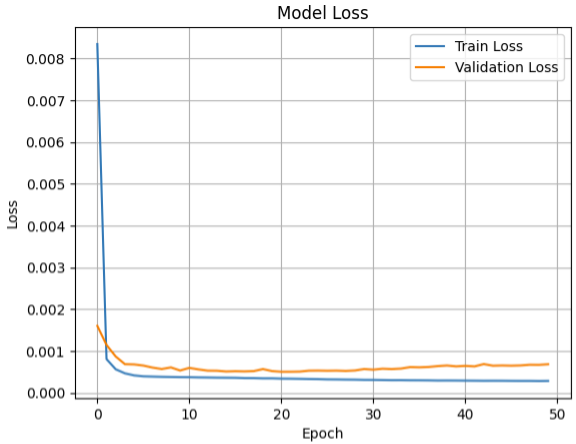
\includegraphics[width=0.45\textwidth]{./afbeeldingen/loss.png}
\captionof{figure}{Training en validation loss van het neuraal netwerk}
\label{fig:train_en_validation_loss}
\end{center}

\subsection{vergelijking met de PID-regelaar}
Om het model te kunnen vergelijken met de traditionele PID-regelaar, zijn beide regelstrategieën getest in dezelfde simulatieomgeving. Hierbij werd gekeken naar de prestaties op responsietijd, stabiliteit, overshoot en robuustheid. In figuur~\ref{fig:vergelijking_met_PID} is een overzicht opgenomen van de meetresultaten. Hieruit blijkt dat het getrainde neuraal netwerk een vergelijkbare prestatie levert als de PID-regelaar in termen van hoogtecontrole van de pingpongbal. Het model wist de gewenste hoogte nauwkeurig te benaderen met een vergelijkbare stabiliteit en minder overshoot in sommige scenario’s. De resultaten van deze vergelijking zijn tevens weergegeven 

\begin{center}
\centering
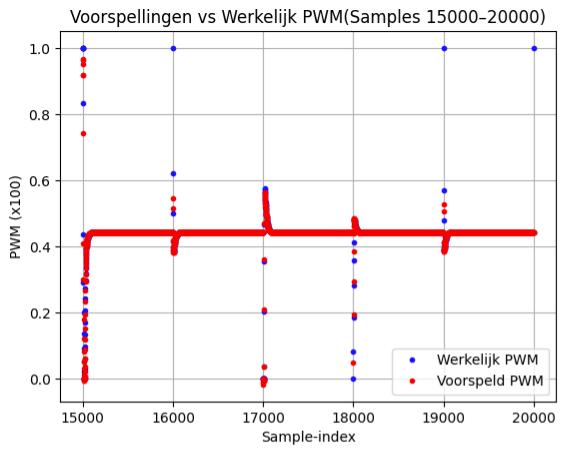
\includegraphics[width=0.45\textwidth]{./afbeeldingen/vergelijking.png}
\captionof{figure}{Vergelijking van de prestaties van het neuraal netwerk en de PID-regelaar}
\label{fig:vergelijking_met_PID}
\end{center}


\subsection{Effect van variatie in data/robuustheid}
In de eerste iteratie van het model werd gekozen voor een grotere netwerkarchitectuur met meerdere verborgen lagen en neuronen per laag. Na overleg met een expert uit het Datalab is besloten om deze complexiteit te reduceren. De reden hiervoor was niet gelinkt aan de beperkingen van de microcontroller, maar aan de aard van het regelprobleem zelf. Het bleek dat het gedrag van een PID-regelaar relatief eenvoudig te modelleren is, waardoor een kleiner model efficiënter bertere prestaties leverde.
Bovendien werd vastgesteld dat een kleinere architectuur minder gevoelig is voor overfitting en beter presteert onder variërende invoerdata. Dit verhoogt de robuustheid van het model, wat essentieel is bij implementatie op fysieke hardware.

\subsection{Observatie tijdens simulatie}
Tijdens de simulaties viel op dat het neurale netwerk in staat was om consistente prestaties te leveren. De stabiliteit en reactietijd bleven binnen aanvaardbare marges. Hoewel deze observaties grotendeels overeenkomen met de bevindingen uit de vorige paragrafen, bevestigen ze de geschiktheid van het model voor real-time regeltoepassingen.



